% Chapter 1

\chapter{Introduction}

\label{intro} 

\graphicspath{{Figures/Introduction}}

\section{From types to program correctness}

In programming language theory and practice, \textbf{static typing} is a widely adopted program validation method where types of expressions are checked against their usage at compile time. Statically typed languages have a long history and are extremely popular, with examples of among both the earliest of programming languages (such as Fortran and ALGOL, \cite{Backus1978-xt}) and the most widely used languages across all platforms  (such as C and its derivatives including Java and C\#, \cite{Ritchie1978-pa}). Static typing is also a core feature of the most advanced and renowned academic languages (such as ML, Haskell, and their derivatives, such as OCaML and Agda, respectively, \cite{Hudak2007-kn}). In practice, statically typed programming languages offer many advantages. Type declarations and annotations add important contextual information about the expected use of variables and expressions. This additional context allows early error detection but also enhances code readability and promotes maintainability, especially in large collaborative projects. The explicit encapsulation of type information in code also creates opportunities for improved tooling through intelligent compiler services and IDE (interactive development environment) support. Additionally, static typing enhances the library documentation by providing clear contracts between library authors and users.

Various approaches to programming language design have embraced different paradigms. Within these paradigms, so-called \textbf{Functional languages} adopt principles based on the mathematical concept of a function. Specifically, functional programming promotes the idea of using functions as the fundamental building blocks of programming and developing abstractions by composing functions. 
Furthermore, so-called `pure' functional programming languages adopt additional rigor from mathematics, such as immutable values (values can not be modified once declared) and referential transparency (functions will always produce the same output when given the same input).  
Like static typing, functional language concepts help programs avoid certain undesired behaviors, such as misaligned pointers and race conditions, by removing or carefully separating the effectful computation from the pure transformation of input and output.
That is, the program can be safely tested and reasoned about, and it takes away the fear that program behavior can be disrupted by external systems, such as network connections or even dates.  For these reasons, functional programming languages are often taught to beginners. Lastly, functional language's strict immutability provides distinct advantages in concurrency and parallelism.


Combining the two disciplines, \textbf{statically typed functional languages} employ both static typing and the principles of functional programming. Most common statically typed function language include Haskell,  ML (with the OCaml dialect being the most popular among the family of ML languages), and F\#. Languages like Idris and Agda even include more advanced type level features like dependent type and session, allowing programmers to express granular check of potential software behavior before running the program. These languages often provide the strongest level of programming safety. It is often advertised that programs in these languages will be error-free if the source code passes the compiling stage, indicating that compilers are able to weed out a large number of programming errors. These safety properties allow statically typed functional languages to be used as proof assistants or formal verification tools. They prove the correctness (or incorrectness) of many systems, from web public key infrastructure \cite{Bhargavan2021-no} to micro-controllers used in space programs \cite{Mokhov2019-zj}. Despite these safety benefits, these languages' presence in the mainstream programming world remains underwhelming. This lack of popularity is often attributed to higher barriers to entry, unfamiliarity, and unforgiving type errors.

One major issue stemming from the promises of statically typed languages is the complexity involved in the systems and tools that safeguard the type-checking process. Ordinarily, this complexity is hidden away from the users. However, most compiler tools fail in usability when they encounter incorrectly typed programs. Many factors contribute to this lack of usability. First, some argue that the expressiveness and power of type systems often come at the cost of usability~\cite{Hage2020-hg}.  Programmers often find type errors hard to read and understand when high-level abstractions such as monads, type classes, and polymorphic types are in play. Second, type errors often use unfamiliar languages with liberal uses of jargon. Last, the type error locations and explanations provided by traditional compiler tools are often misleading or wrong. All these factors make debugging type errors notoriously difficult.

\section{The Open Challenges Of Type Errors}

Type errors can be notoriously difficult to understand and use, particularly for newcomers to programming or when using a language that is particularly strict about types. Type errors are often believed to be a major contributor to static typing's reputation of being a high barrier to entry. I believe it is important to understand the root of the challenges of using type errors in order to address them. To achieve that, I believe it is useful to put type errors in proper context, more specifically, comparing them with other classes of programming errors (parsing errors, runtime errors). 

\subsection{Types Are As Complex As Runtime Values}

Unlike expressions (values and variables) of a program, Types are computed at compile time. However, similar to evaluation semantics, the type checking computations can be complex. In fact, in many programming languages, type checking is shown to be non-terminating and Turing complete~\cite{Wells1999-ob}. This raises the challenge of explaining such a complex computing process when programmers are burdened to correct ill-typed programs. Type checking cannot be inspected using conventional tools. Inserting print statements inside type annotation is not possible. 


\subsection{Clues For Type Checking Are Implicit}
Understanding how types are assigned in a program becomes more challenging when the programming language uses type inference.  Type inference \cite{Damas1982-sc},  also known as implicit typing,  is a technique that allows programmers to omit the ritual of writing type annotations altogether, and the type checker will infer the most general types (principal types) for each expression. Even for languages that don't employ implicit typing, some typing rules are hidden from programmers.
For example, the \texttt{if} expression in many programming languages. The semantics is very clear, but the typing rules are hidden.

\begin{figure}[hbt]
  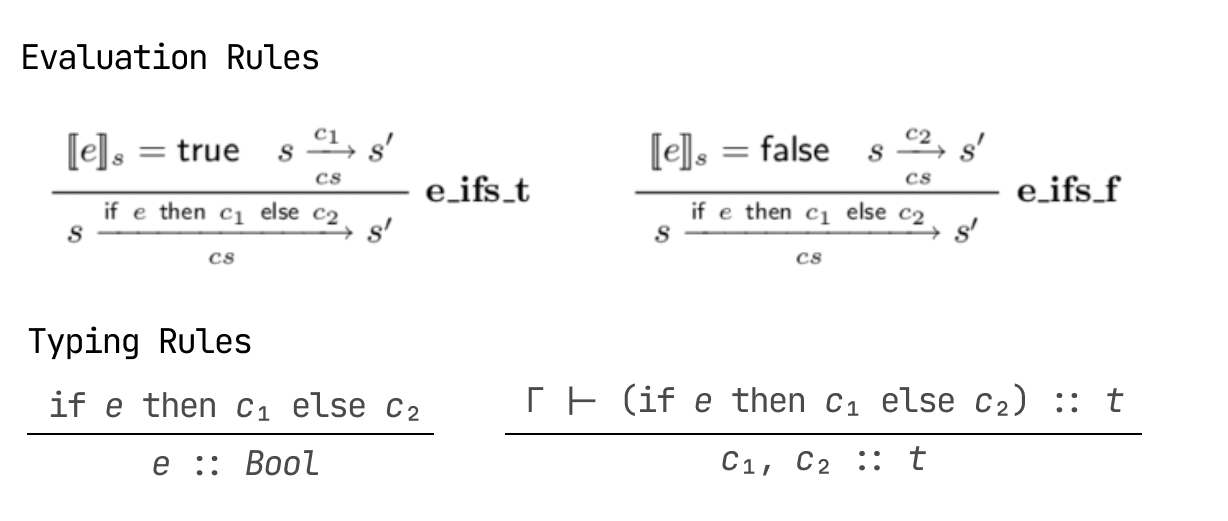
\includegraphics[width=\linewidth]{IfRules.png}
  \caption{
   The evaluation rules and typing rules of if expression in a typical programming language.
    }
\end{figure}


\subsection{Lack of tool support}
Lastly, few tools are dedicated to supporting type errors. Runtime programming errors have been studied extensively as a research subject, and numerous industry tools are focused on understanding and solving runtime errors(GDB, breakpoints.) However, in comparison, tool support type errors remain the same depth and capability as they were many decades ago. Most programming environments render type errors verbatim to the terminal.   


\begin{figure}[hbt]
  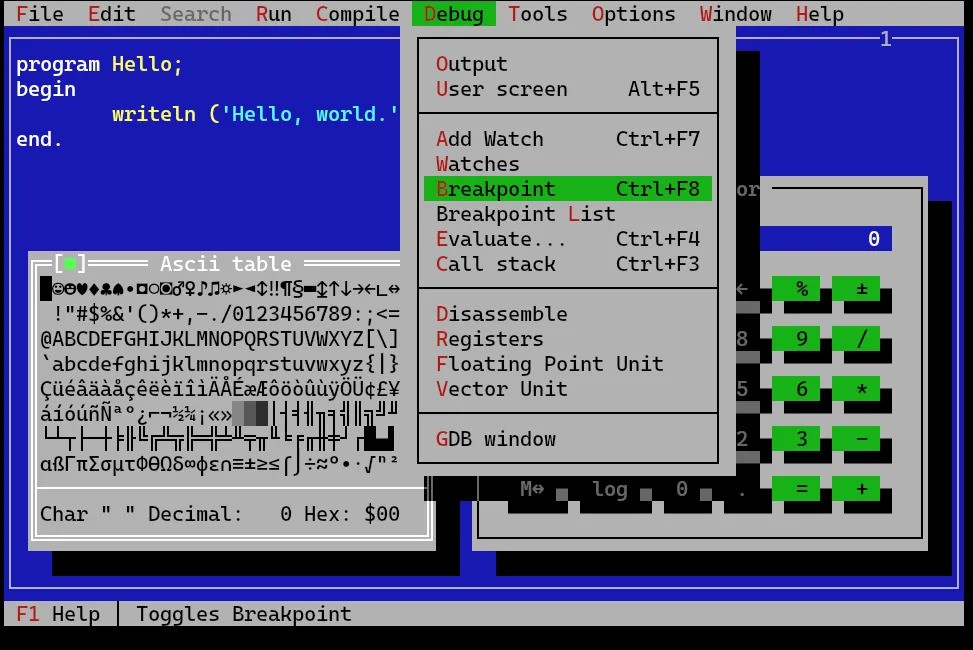
\includegraphics[width=\linewidth]{FreePascal.jpg}
  \caption{
    Run time debugging using break point in the Free Pascal interactive development environment in 1997
    }
\end{figure}

\begin{figure}[hbt]
  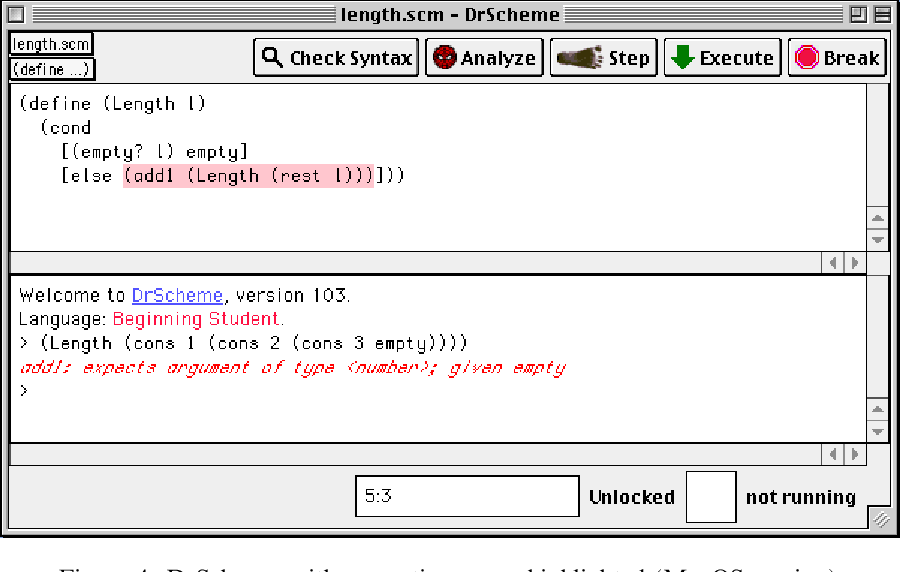
\includegraphics[width=\linewidth]{DrScheme}
  \caption{
    Dr Scheme, an interactive development environment for the Scheme language, highlights a runtime error
    }
\end{figure}

My research is motivated by the inherent difficulties in debugging type errors and the dormant development of improving type errors using modern graphical capabilities and HCI techniques.

\section{Research Aim}

\subsection{Aim 1. Develop a Comprehensive Understanding of the Knowledge Required by Programmers to Understand and Resolve Type Errors.}

To date, there is no unified representation of type errors. However, most contemporary compiler tools represent type error as the combination of three objects: a location where the failed type checking failed, an expected input, and the actually encountered input.

\subsubsection{Objective 1.1 To Identify and Accurately Report Multiple Locations Contributing to Type Errors.}

Traditional tools are limited to reporting a single location for a type error, which many researchers have addressed as an unhelpful limitation. Programmers are often unable to find a resolution at the reported location and are forced to expand their search without guidance. We want to improve this by reporting accurate locations relevant to the type of error.

\subsubsection{Objective 1.2 To Communicate that there may be more than one explanation for a type error}

Erroneous programs can often be explained in multiple ways. When two pieces of evidence contradict each other, traditional tools choose the first one they encounter as the truth and the second one the culprit. When a contradiction consists of more than two pieces of evidence, traditional tools will generally ignore everything after the infeasibility is encountered. To improve this, first, we want to preserve the multiple explanations of type errors without picking sides. Second, we want to take into account all evidence.

\subsubsection{Objective 1.3 To Communicate That There May Be More Than One Cause Of A Type Error}

Type error does not end with a location in the source code. Programmers can still struggle to resolve a type error even after reaching the exact location of the culprits, failing to understand the logical explanation of the type error. Internally, type errors can be caused by mismatched types, unfulfilled type class constraints, or trying to construct infinite types. Externally, type error can be caused by typos, outdated type annotation, incomplete implementation, too few or too many arguments in a function application, etc.. Helping programmers find the cause or provide an accurate inference of what is the cause of the type error.

\subsection{Aim 2. Support Resolution Of Type Errors Through Modern Programming Environments.}

To integrate rich type error data into a modern, visual programming environment and workflow that allows people to work more efficiently with strongly typed languages.


When humans are put in the middle, more information does not equal better comprehension. With enriched data representation, we want to deliver type errors to better support programmers’ comprehension and the chance for a successful resolution.

\subsubsection{Objective 2.1 Communicate the key concepts of type errors effectively using modern programming tools}

The concepts of type errors are traditionally displayed as text. These concepts include error locations, alternative explanations, causes, and intermediate type signatures. We explore more intuitive techniques and media to communicate these concepts to better facilitate comprehension.

\subsubsection{Objective 2.2 Use Interactive Tools for Investigating and Resolving Type Errors.}

To avoid presenting overwhelming information, we explore different techniques of interactively exploring the type errors. These techniques include dividing the type error into small chunks that follow a linear line of reasoning or bisecting the error one step at a time into smaller concepts.


\section{Contributions}

\subsection{A categorization of type errors based on the structure of the evidence of a type error}

A \textbf{multi-step type error} is a type error that involves multiple inference steps between the two endpoints. An important challenge with multi-step type errors is to convey the logical relation of every location while presenting infeasibility. 

A \textbf{multi-witness type error} is a type error that involves multiple endpoints supporting the same typing possibility. With multi-witness type error, it is harder to focus on the logical relation of every location as the complexity grows exponentially as the number of witnesses increases. Rather, it is more helpful to identify the two typing possibilities and the endpoint locations that support them.

A \textbf{multi-party type error} is a type error that involves more than two typing possibilities. The multi-party type error is thought to be less intuitive and harder to comprehend. The most prominent task is to separate the type error into simpler type errors. 


With this classification, I contributed two systems -- Chameleon and Goanna -- to address the challenges of type error debugging in different error categories.

\subsection{Explaining Multi-Step Type Errors Through Chain-Of-Thought Visualization}

\subsubsection{Technical Contribution - Chameleon}
We contribute Chameleon, an interactive Haskell type error debugging tool. Internally, Chameleon computes all relevant locations that contribute to the type of error. Via a set of iteratively designed interfaces, Chameleon preserves the two alternatives of the type error and the supporting evidence for each.

\subsubsection{An evaluation on how programmers use type error slicing and chain of thought visualization to understand type errors}
We contributed a series of studies of the effects of debugging with visual representation of types and interactively explored type errors. We show that there is a difference between using traditional tools and enhanced type error debugging tools like Chameleon. And we show that this difference is more significant when debugging complex type errors.

\subsection{Iterate potential causes of multi-witness and multi-party errors}

\subsubsection{Technical Contribution -- Goanna}

We contribute Goanna, a Haskell type error debugging tool. 

Like Chameleon, Goanna iterates relevant locations that contribute to the type error and presents alternatives to the type error. 

Different from Chameleon, Goanna will exhaust all possible alternative explanations of the type error. Also, Goanna presents a type error by dividing it into a list of potential causes and their respective fixes. With Goanna, Haskell programmers can resolve type errors by exploring a list of potential root causes of errors. These causes are ordered using our heuristics so that the more likely causes are on top. We show that via our empirical evaluation, Goanna outperforms existing Haskell compilers when explaining the type error, with the slight disadvantage of an increased computation time.

\subsubsection{An evaluation on accuracy, conciseness, and performance of MCS-based type debugging and our heuristics}

We evaluated Goanna's effectiveness using 86 diverse Haskell programs from online discourse, demonstrating its ability to accurately identify and resolve type errors. Additionally, we present a collection of techniques and heuristics to enhance Goanna's suggestion-based error diagnosis and show their effectiveness from our evaluation.


\subsection{Visualizing Types}

\subsubsection{Technical Contribution -- GeckoGraph}

In addition to the two systems, I also contribute GeckoGraph, a graphic notation for Haskell types. GeckoGraph describes the same information as a type signature does but uses colors, shapes, and symbols to make certain structures easy to identify at a glance. GeckoGraph is designed to use visual elements to improve the understanding of type-level concepts. This includes type classes, parametric type variables, and high-rank types. When used to compare two types, GeckoGraph helps clarify differences visually. It makes errors like too few or too many arguments in applications and unmet type class constraints obvious.

\subsubsection{An evaluation on how programmers use graphic type notation}

We conducted a large-scale study on the effectiveness of using GeckoGraph to perform a series of Haskell tasks. We concluded that with GeckoGraph, programmers are able to succeed in harder tasks.

% \section{Research Method}

% \subsection{Human-centered programming language studies}

% One important decision that shape a lot of my work is employing human-centered research methods with our novel programming language systems. The adopting of human-centered methods happens at every stage of the projects: prototyping, development and evaluation. Although the using of these methods are not new at all, but they certainly are not the most polular choices in programming language studies.

% The motive of such decision is that it is impossible to understand what are the good qualities of type errors without observing how human use type errors to gain understanding. 


% The downside of study programming language is iterative design is very hard. programming tasks involves complex inputs and outputs, and it is very hard to study an incomplete system without a fully working systems. For instance, if we are to study the effect of type errors, it is most effective to have a system that can recognize type-correct program from ill-typed one. It is hard to evaluate with a mock-up or wizard of oz style fake outputs to study users' interaction.  To address this limitations, we have a few ideas implemented in our research:

% A minimal but practical set of language 
% Design for human from start



\section{Thesis outline}

The thesis can be divided into two parts. The first part (Chapters 1, 2, and 3) surveys the vivid panorama of type systems and programming languages. The purpose of these chapters is: 1. to situate the work I will illustrate in later chapters, 2 to introduce the proper definitions and terminilogies I use in this thesis.  The second part (Chapters 4, 5, 6, and 7) delves into three individual pieces of work, each targeting a specific problem in type error debugging.


% \subsection{Chapter 2}

% Chapter 2 introduce the development of two programming features: functional programming and static typing. We started by introducing the evolutions functional programming and static typing. We discuss their counterparts and the arguments against them. We then discuss the important milestones in improving compiler type error messgaes. We discuss the emerging demmand of these tools of programming robust code, as the way we program altered by the seismic impact of large language models.  


\subsection{Chapter 2}
We provide some technial background in Chapter 3. This include the tradiional methods of Haskell type checking and constraint based type inference. Follow this thread, we continue to discuss the tools and techniques in constraint satisfiability analyasis that we use to improve type error reprotiong in later chapters. Last, we give the categorization of type errors and their examples. 

\subsection{Chapter 3}
This chapter introduces the work related to our implementation of Chameleon and our study on its effect on debugging type errors. This chapter starts with an introduction of our motivation, succinctly summarised in three characteristics of bad-type error messages. We then introduce Chamaleon by imagining ourselves as hypothetical programmers combating Haskell-type errors, luckily with the help of Chameleon. We go on to introduce the system design and iterative prototyping methods used to develop Chameleon. Lastly, our series of experiments on Chameleon's effect on solving type errors compared to traditional compiler tools. 


\subsection{Chapter 4}

The work we discuss in Chapter 5 is about Goanna. Goanna is a Haskell type-error debugger we developed. In this chapter, we first report some common limitations of traditional compiler error messages. We then go on to showcase how Goanna Fix type errors are able to address these limitations in a few examples of realistic type errors.  Next, we discuss the implementation of Goanna and our heuristics for ranking potential causes and identifying unhelpful suggestions. Last, we show our empirical study of the accuracy, conciseness, and performance of Goanna using a collection of real-world Haskell type errors. 

\subsection{Chapter 5}

In this chapter, we discuss our work on visualizing type annotations. In this, we showed our work in GeckoGraph and our empirical study on its effect. We start by presenting some usability challenges in using polymorphic types. We then describe the design goal of GeckoGraph and how it can be constructed from a textual type annotation using a few construction rules. We then show our large-scale study on the effect of using visual type annotations in programming and solving type errors. 


\subsection{Chapter 6}

In the last chapter, we reiterate our contributions with more remarks on their contexts. We discuss a few directions for future work. This includes the direction in future tool development, as well as future research opportunities. Lastly, in closing words, we return to the map field of programming language and the vast uncharted area of the future of programming. 